\documentclass[a4paper,11pt]{article}
%\hyphenpenalty 10000
\usepackage[utf8]{inputenc}
%\usepackage[T1]{fontenc}
\usepackage{amsmath,amssymb}
\usepackage[english,french]{babel}
\usepackage[pdftex]{graphicx}
%\usepackage[options]{mcode}
\usepackage{textcomp}
\usepackage{array}
\usepackage{subfig}
\usepackage[left=2cm, right=1cm, bottom=2cm, top=2cm]{geometry}
\usepackage{float}
\usepackage{multicol}
\usepackage{tabularx}
\usepackage{fancybox}



\usepackage{color} % gestion de différentes couleurs

\definecolor{linkcolor}{rgb}{0,0,0.6} % définition de la couleur des liens pdf
\usepackage[ pdftex,colorlinks=true,
pdfstartview=FitV,
linkcolor= linkcolor,
citecolor= linkcolor,
urlcolor= linkcolor,
hyperindex=true,
hyperfigures=false]
{hyperref} % fichiers pdf 'intelligents', avec des liens entre les références, etc.

\usepackage{fancyhdr} % entêtes et pieds de pages personnalisés 
\pagestyle{fancy}
\fancyhead[L]{\scriptsize \textsc{Etude théorique de la translocation de
biomolécules à travers un nanopore}}
\fancyhead[R]{\scriptsize \textsc{Menais Timothée}}
\fancyfoot[C]{ \thepage} 

\begin{document}



% Pour faciliter la mise en forme de la page du titre, on supprime l'indentation automatique en début de paragraphe
\setlength{\parindent}{0pt}

% Pas d'en-tête ni de pied pour la première page
\thispagestyle{empty}


\includegraphics[height=2cm]{phelma.jpg} \hfill 
\includegraphics[height=2.2cm]{cea.jpg} \hfill 
\includegraphics[height=2cm]{ujf.jpg}

\vspace{0.5cm}

\begin{tabularx}{\textwidth}{@{} l X l @{} }
{\sc Master  2R EP} & & Projet bibliographique 2012 \\
{\it Grenoble INP - PHELMA} & & Menais Timothée \\

\end{tabularx}

\begin{center}

\vspace{1.5cm}

\rule[11pt]{5cm}{0.5pt}

\textbf{\huge Etude théorique de la translocation de
biomolécules à travers un nanopore.}

\rule{5cm}{0.5pt}

\vspace{1.5cm}

\parbox{15cm}{\small
\textbf{Abstract} : \it Projet bibliographique, Timothée Menais, M 2R EP, 2012.

\vspace{0.5cm}
\rm Durant mon stage, j'étudierai d'un point de vu analytique et numérique la translocation (passage) de biomolécules (principalement de l'ADN simple brin) à travers un nanopore de graphène, au sein du Groupe Théorie, SPrAM, INAC du CEA de Grenoble. Intéressante d'un point de vue fondamental, cette étude peut également avoir des retombées importantes pour la compréhension de phénomènes biologiques et des applications techniques notamment pour le séquençage de génomes. Des outils théoriques de physique statistique et numériques de dynamique moléculaire seront mis en œuvre afin de comprendre le rôle et l'importance de la structure du polymère et des forces appliquées sur le temps nécessaire à la translocation. De récentes expériences utilisant des pores dans une mono-couche de graphène ont produit des résultats encourageants qui nous poussent à concentrer notre étude sur la compréhension et la modélisation de ces nouveaux pores.
} %fin de la commande \parbox du résumé


\vspace{0.5cm}

\parbox{15cm}{
\textbf{Mots clés : \it ADN, Graphène, Dynamique moléculaire, Physique statistique.} }%fin de la commande \parbox des mots clefs

\vspace{0.5cm}

\parbox{15cm}{
Stage encadré par :

{\bf Dr Arnaud Buhot }

\href{mailto:	arnaud.buhot@cea.fr }{\tt 	arnaud.buhot@cea.fr }  / tel: ++33 438 78 38 68

%{\bf Dr Ulrich Keyser}

%\href{mailto:	ufk20@cam.ac.uk}{\tt 	ufk20@cam.ac.uk} / tel: +44 (0)1223 337272

Groupe Théorie

Structures et Propriétés d'Architectures Moléculaires

Institut Nanoscience et Cryogénie
{\it 

17 rue des Martyrs
38054 Grenoble cedex 9
France}

\url{http://inac.cea.fr/spram/Phocea/Vie_des_labos/Ast/ast_groupe.php?id_groupe=397}
} %fin de la commande \parbox encadrant / laboratoire d'accueil

\vspace{1cm}



\includegraphics[height=1.8cm]{spram.jpg} \hspace{0.3cm}

\includegraphics[height=1.8cm]{inac.jpg}

\end{center}
\selectlanguage{french}

\begin{flushright}
\today
\end{flushright}

\vfill
\hfill 

% Pas d'entête ni de pied pour la page de sommaire



\setlength{\parindent}{10pt}



\section*{Introduction}


La translocation de biomolécules à travers un nanopore est un domaine scientifique très actif tant sur le plan expérimental que sur le plan théorique. Ceci est principalement dû aux applications potentielles en biotechnologies et en médecine, notamment le séquençage rapide et économique envisagé lors de la translocation de brins d'ADN.\\

L'aspect appliqué est important mais ce problème soulève aussi des questions fondamentales très intéressantes sur le comportement de polymères quand ils sont confinés.\\

De récentes expériences de translocation mettent en œuvre des nanopores creusés dans des couches monoatomique de graphène. Le graphène, isolé pour la première fois en 2004, est un cristal aromatique bidimensionnel de carbone dont l'empilement de plusieurs plans forme le graphite. Ces expériences contournent les problèmes d'épaisseur inhérents aux autres types de pores.\\

Le but de mon stage est de modéliser la translocation d'ADN simple brin à travers un nanopore de graphène en caractérisant le temps de translocation, l'influence des propriétés du graphène et discuter de l'éventuelle possibilité de séquençage.\\

Notre étude théorique de la translocation de biomolécules à travers un nanopore s'articulera autour d'un premier chapitre présentant les outils analytiques de physique statistique mis à contribution, d'un second chapitre portant sur la modélisation numérique de dynamique moléculaire, et d'un dernier chapitre traitant de résultats expérimentaux et de l'introduction du graphène.



\tableofcontents



\newpage 

\section{Outils analytiques}

Dans cette partie nous allons développer les outils analytiques de physique statistique nécessaires pour aborder le comportement des polymères et ce notamment lors de la translocation.

\subsection{Polymères idéaux et non idéaux}
Nous allons dans un premier temps présenter un modèle naïf de polymère idéal  présenté dans la thèse de Henk Vocks \cite{these} afin d'avoir une idée générale de la situation et de reposer quelques bases de physique statistique.\\

Le polymère évolue sur un réseau périodique carré de paramètre $\lambda$. La tête du polymère est placée sur un des nœuds du réseau. Les monomères consécutifs sont placés sur un des $z$ ($z=4$ pour un réseau carré) sites plus proches voisins, le polymère réalise alors une marche aléatoire (Figure \ref{resideal}).

\begin{figure}[H]
\begin{center}
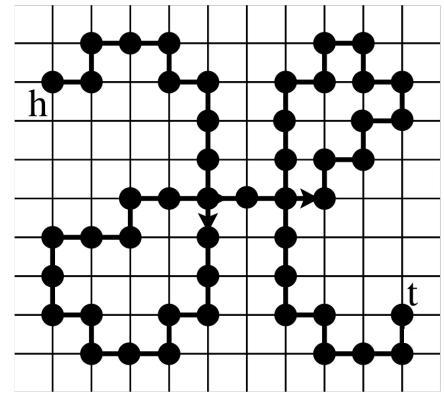
\includegraphics[width=0.33\textwidth]{resideal.jpg}

\caption{Réseau carré montrant la marche aléatoire du polymère.}
\label{resideal}
\end{center}
\end{figure}

On déduit facilement que pour un degré de polymérisation $N+1$, il y a $Z_{ideal}=z^N$ polymères distincts possibles. Rappelons des résultats concernant la marche aléatoire: soit $\textbf{r}$ le vecteur position du marcheur par rapport à l'origine, $<\textbf{r}>=0$ et $<\textbf{r}^2>=d^2 t$ avec $d$ la taille d'un pas et $t$ le nombre de pas effectués. Ici $t=N$ d'où une taille moyenne du polymère $R_0=\lambda N^{\frac{1}{2}}$.\\

Afin de trouver l'énergie libre correspondant à chaque conformation, on établit une équation différentielle sur la probabilité, $P(\textbf{r},N)$, d'un monomère d'être en $\textbf{r}$, car en introduisant $\textbf{b}_i$ les z vecteur plus proches de la position $\textbf{r}$:
\begin{center}

$P(\textbf{r},N)= \frac{1}{z}\sum_{i=1}^{z} (P(\textbf{r}-\textbf{b}_i,N-1)$\flushright(1)

\end{center}

L'équation (1) est linéarisée, l'équation différentielle obtenue est résolue et l'énergie libre est donc:
\begin{center}

$F(r) = -K_B T ln(P(r,N)) = F(0) + \frac{3 K_B T \textbf{r}^2}{2 R_0^2}$\flushright(2)

\end{center}
Avec $K_B$ la constante de Boltzmann et $T$ la température thermodynamique (voir la thèse de Vocks \cite{these}).\\

Bien entendu ce modèle est simpliste, un vrai polymère ne peut en aucun s'intersecter lui même, les monomères peuvent être différents, ou encore des forces peuvent être appliquées.\\

 Le lecteur intéressé trouvera un exemple de polymère non idéal développé dans la thèse de Vocks \cite{these}, exemple incluant la condition de non intersection (self avoiding walk) ainsi que des interactions répulsives entre monomères pour déduire une forme différente de l'énergie libre ainsi qu'une taille dépendant maintenant de l'exposant de Fleury ($N^{\nu}$ avec $\nu=\frac{3}{5}$) et non plus de $N^{\frac{1}{2}}$.

\subsection{Eléments dynamiques}

Nous allons maintenant proposer (comme dans la thèse de Vocks \cite{these}) un modèle permettant d'aborder la dynamique d'une chaine. Il s'agit du modèle de Rouse (Figure \ref{rouse}).

\begin{figure}[H]
\begin{center}
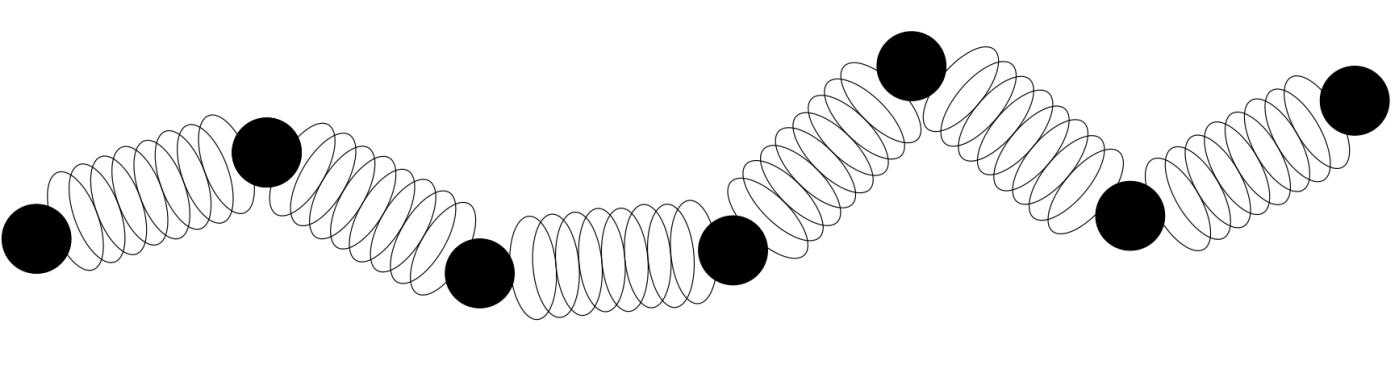
\includegraphics[width=0.75\textwidth]{rouse.jpg}

\caption{Modélisation du polymère par une chaine d'oscillateurs.}
\label{rouse}
\end{center}
\end{figure}

Le polymère est modélisé par une chaine d'oscillateurs (de type billes/ressorts). Physiquement, le ressort ne représente pas une liaison entre monomères mais plutôt une partie du polymère assez longue pour que la statistique gaussienne puisse lui être appliquée. De l'équation (2) obtenue précédemment on déduit l'énergie élastique du ressort connectant les billes $n$ et $n+1$ séparées par une distance d'équilibre moyenne $\lambda$:

\begin{center}

$F_{n,n+1} = \frac{3 K_B T}{2} \frac{(\textbf{r}_{n+1}-\textbf{r}_n)^2}{\lambda^2}$\flushright(3)

\end{center}

L'énergie élastique totale du polymère est alors la somme des contributions séparées:
\begin{center}

$F_{tot} = \sum_{n=0}^{N-1} F_{n,n+1}$\flushright(4)

\end{center}

En dérivant cette énergie, on obtient la force élastique exercée sur une bille. Le polymère évolue dans un solvant, il y aura donc une force de frottements visqueux et de plus le mouvement brownien va aussi devoir être pris en compte. L'équation du mouvement est donc la suivante:

\begin{center}

$m \frac{d^2 \textbf{r}_n}{dt^2} = -\frac{\partial F_{tot}}{\partial \textbf{r}_n} -\epsilon \frac{d \textbf{r}_n}{dt} +\epsilon \textbf{g}_n$\flushright(5)

\end{center}

Avec $\epsilon$ le coefficient de frottement et $\epsilon\textbf{g}_n$ la contribution brownienne, une force de moyenne nulle et de variance $ 2 K_B T$.\\



Comme nous nous situons à une échelle nanométrique, le nombre de Reynolds\footnote{Le nombre de Reynolds est le rapport des échelles de temps caractéristiques inertielles et visqueuses} de l'écoulement va être très faible, ce qui permet de négliger les termes inertiels et d'obtenir ainsi l'équation de Langevin, résultat de l'équilibre des forces avec le Stokes drag:

\begin{center}

$\frac{d \textbf{r}_n}{dt} = -\frac{1}{\epsilon}\frac{\partial F_{tot}}{\partial \textbf{r}_n} +\textbf{g}_n$\flushright(6)

\end{center}

Cette équation est résolue en faisant passer $n$ de valeurs discrètes à des valeurs continues (détails dans la thèse de Vocks \cite{these}). Il faut principalement retenir que le déplacement carré moyen du centre de masse:

\begin{center}

$<(\textbf{r}_{CM}(t)-\textbf{r}_{CM}(0))^2>=\frac{6 K_B T}{N \epsilon} t = 6 D_R t$\flushright(7)

\end{center}

Et le fait que le coefficient de diffusion $D_R$ soit proportionnel à $N^{-1}$. Pour un monomère, le déplacement carré moyen à temps long est la somme de celui du centre de masse et d'une constante multipliée par $N$, à temps court il croit en $t^{\frac{1}{2}}$.\\

Il est intéressant de noter que le temps de relaxation nécessaire au centre de masse pour parcourir sa longueur est alors proportionnel à $N^2$ (ou $N^{1+2\nu}$ dans le cas non idéal). Ce qui n'est pas observé expérimentalement à cause des interactions hydrodynamiques.



\subsection{Translocation}

La translocation d'un polymère est son passage d'un compartiment cloisonné à un autre par un pore les reliant. La molécule passe d'un coté appelé cis à l'autre appelé trans en deux temps. Le premier temps consiste en ce qu'une extrémité de la chaine atteigne l'entrée du pore. Cette probabilité et le temps qui lui est associé peuvent être estimés analytiquement et ne présentent pas de défi \cite{milchev}. Le second temps représente la translocation en elle même (voir Figure \ref{transloc}), il s'agit du temps pendant lequel le polymère occupe le pore.\\

\begin{figure}[H]
\begin{center}
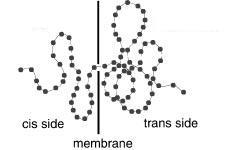
\includegraphics[width=0.35\textwidth]{transloc.jpg}

\caption{Un polymère en cours de translocation.}
\label{transloc}
\end{center}
\end{figure}



Ce second temps, appelé temps de translocation ($\tau$) est très important puisqu'il représente dans beaucoup de cas une des seules mesures expérimentales accessibles.\\

La translocation peut se dérouler dans différents contextes. Elle peut être due uniquement aux fluctuations thermiques, on parle alors de translocation non biaisée, ou être pilotée par une force extérieure, on parle alors de translocation forcée (driven translocation). Les forces extérieures peuvent être de natures variées, on citera notamment l'utilisation de champs électriques (électrophorèse), de gradients de potentiels chimiques, de flux imposé sur le solvant, ou encore l'emploi de pinces optiques.\\

Le temps de translocation dépend alors fortement de la taille du polymère et de la force appliquée, d'une façon générale on a:

\begin{center}

$\tau = N^\alpha f^{-\delta}$\flushright(8)

\end{center}

Il faut alors déterminer $\alpha$ et $\delta$.\\

La première étape consiste à déterminer la forme de la barrière énergétique à franchir au cours de la translocation. Deux démonstrations intéressantes sont présentées respectivement dans la thèse de Vocks \cite{these} et dans un article de Sung et Park \cite{sung}.\\

Dans le premier exemple, Vock invoque la modification de la fonction de partition due aux contraintes topologiques imposées par la présence du pore et de la cloison:\newline$Z_{non ideal} = \tilde{z}^N N^{\gamma-1}$ devient $Z^{cloison}_{non ideal} = \tilde{z}^N N^{\gamma_1-1}$ La fonction de partition totale étant alors le produit $Z^{cloison}_{non ideal}(n) Z^{cloison}_{non ideal}(N-n)$ avec $n$ le nombre de monomères du coté trans.\\

L'énergie libre alors dérivée est de la forme:

\begin{center}

$F(N,n) = K_B T [(1-\gamma_1)ln[n(N-n)] - Nln(\tilde{z})]$\flushright(9)

\end{center}

Dans leur article, Sung et Park \cite{sung} s'affranchissent de la contrainte du réseau et dérivent une forme similaire uniquement avec des probabilités (le terme $Nln(\tilde{z})$ est alors défini comme une constante puisqu'il modifie la hauteur de la barrière énergétique mais pas sa forme vis à vis de la coordonnée réactionnelle).\\

A cette énergie libre, appelée barrière entropique (la barrière est due uniquement aux restrictions topologiques et n'a pas de contribution enthalpique, d'où le terme entropique)  peuvent s'ajouter des potentiels dus aux forces appliquées, la Figure \ref{transpot} présente la forme de la barrière avec différents potentiels ajoutés:

\begin{figure}[H]
\begin{center}
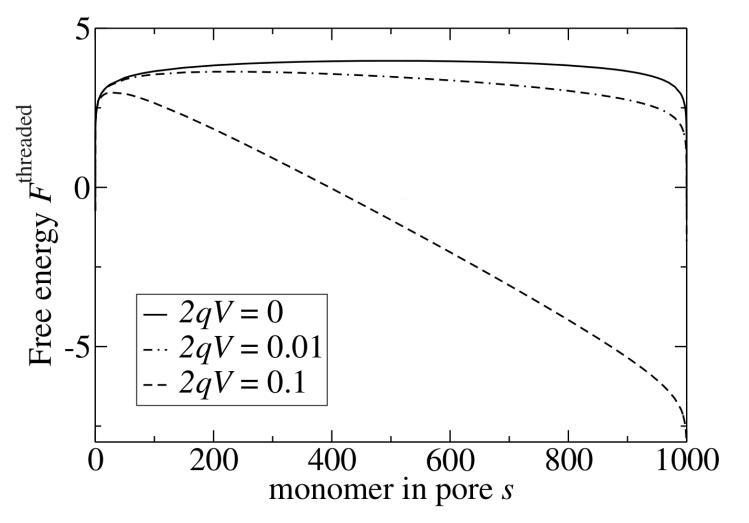
\includegraphics[width=0.52\textwidth]{transelec.jpg} 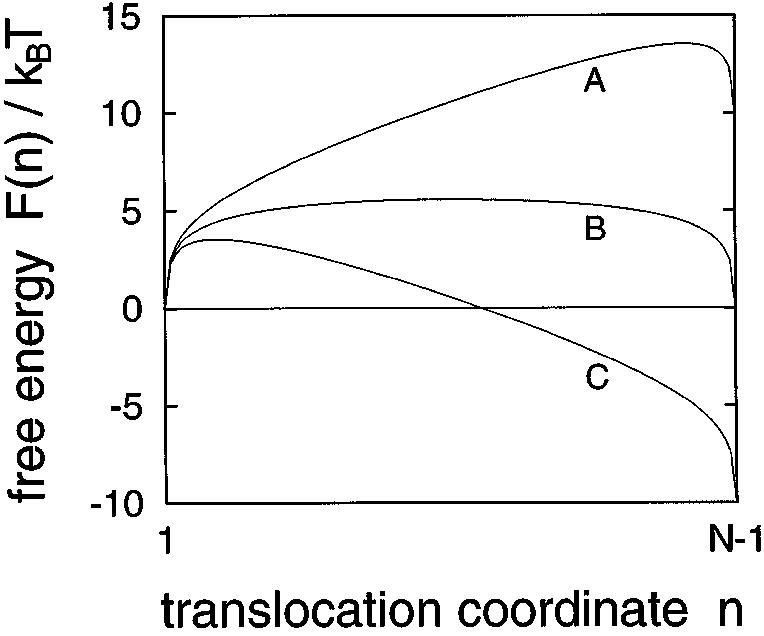
\includegraphics[width=0.42\textwidth]{transpotchim.jpg}

\caption{A gauche: Influence d'un potentiel électrique sur la barrière énergétique \cite{these}.
A droite: utilisation d'une différence de potentiel chimique (A et C) \cite{sung}.}
\label{transpot}
\end{center}
\end{figure}

Une fois les contraintes énergétiques connues, la translocation est traitée comme un processus de diffusion aléatoire gouverné par l'équation de Fokker-Planck. Il s'agit d'une équation différentielle sur les probabilités, le développement des calculs est réalisé dans l'article de Sung et Park \cite{sung} ainsi que dans l'article de review de Milchev \cite{milchev}. Pour en comprendre vraiment l'origine, il est conseillé de se plonger dans un ouvrage complet de physique statistique.\\

On retiendra le résultat général pour la translocation non biaisée: $\tau$ est proportionnel à $N^{1+2\nu}$. Les valeurs relatives de potentiel introduit par une force et des fluctuations thermiques (de l'ordre de $K_B T$) va influer sur les valeurs de $\alpha$ et $\delta$\cite{milchev,sung}.\\

Il est également intéressant de noter l'influence des interactions hydrodynamiques présentées dans la review de Milchev \cite{milchev}. La dernière partie de l'article de Sung et Park \cite{sung} présente l'influence purement entropique des protéines chaperones lors de la translocation.\\

On notera également l'originalité d'un article publié par Arnold J Storm and co-authors \cite{storm} qui présente deux forces (champ électrique et Stokes drag) opposées lors de la translocation.



\newpage 

\section{Dynamique moléculaire}

Dans le cadre de mon projet de stage, nous envisageons une approche assez différente des simulations classiques sur réseau avec maillage comme c'est souvent le cas en mécanique des fluides ou dans certains travaux sur les polymères comme dans la thèse de Vocks \cite{these}. Nous proposons de modéliser les différentes parties du polymère, les champs de force et intégrer numériquement les équations du mouvement, c'est ce qu'on appelle faire de la dynamique moléculaire.

\subsection{Le système biologique}

Il est primordiale afin de décrire au mieux la réalité physique, de comprendre ce qui constitue le système étudié: l'ADN.\\

L'ADN est le support de l'information génétique du vivant. Il s'agit d'un bio-polymère constitué d'une séquence de quatre monomères différents. Ces monomères, appelés nucléotides sont constitués de phosphate, de sucre et d'une base azotée, seul élément distinct entre nucléotides: l'adénine, la cytosine, la guanine et la thymine (l'uracile présente uniquement en substitut de la thymine dans l'ARN ne sera pas abordée ici). Il se trouve dans les cellules, contenu généralement dans le noyau. La translocation de l'ADN est le mécanisme impliqué dans nombre d'infections virales et pourrait être utilisé pour la thérapie génique.

\begin{figure}[H]
\begin{center}
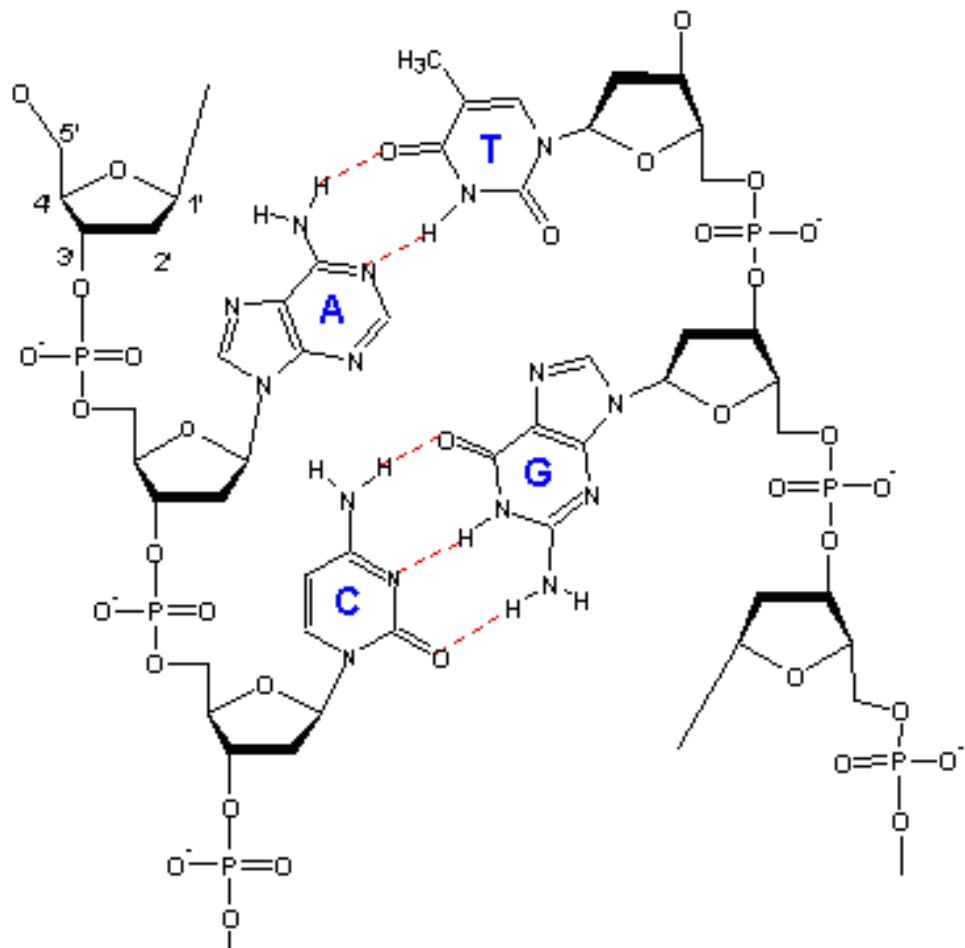
\includegraphics[width=0.6\textwidth]{adn.jpg}

\caption{Structure chimique de l'ADN. Le squelette est composé d'une succession de phosphates et de sucres, à chaque sucre est liée une base azotée. Les bases azotées peuvent interagir par liaisons hydrogènes.}
\label{adn}
\end{center}
\end{figure}

La structure chimique de l'ADN est aujourd'hui parfaitement connue (Figure \ref{adn}), la nature des liaisons et interactions ne sont plus mystérieuses. Numériquement, il est impossible de faire converger les calculs en modélisant chaque atome et chaque interaction, la difficulté de modélisation sera de réduire le modèle sans exagérations pour que les calculs soient réalisables et conservent un sens physique. 

\newpage

\subsection{La modélisation}

Afin de créer un modèle numérique fiable et robuste, il convient de décomposer chaque monomère en sous système. Il semble naturel de faire une décomposition en sucre, phosphate et base azotée comme l'on fait Margaret C Linak and co-authors \cite{jchem}. Leur résultats étant fiables, nous envisageons de nous inspirer fortement de la manière dont ils ont modélisé l'ADN simple brin (Figure \ref{dnamod}).
\begin{figure}[H]
\begin{center}
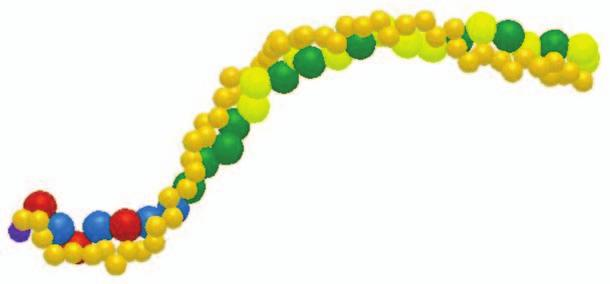
\includegraphics[width=0.6\textwidth]{dnamod.jpg}

\caption{Chaine de nucléotides avec trois composants: sucres, phosphates et bases azotées\cite{jchem}.}
\label{dnamod}
\end{center}
\end{figure}

Une fois ce découpage préparé, l'étape suivante consiste à définir tous les potentiels d'interaction entre tous les éléments.\\

Dans leur papier, Margaret C Linak and co-authors \cite{jchem}, définissent plusieurs types de potentiels à partir d'étalons de distance ($\sigma$, $R_0$ et $\gamma$) et d'énergie ($\epsilon$):

\subsubsection*{Les interactions non spécifiques:}

Il s'agit d'une part des interactions de type volume exclu, modélisées par un potentiel de Lennard-Jones:

\begin{center}

$U_{EV}(r_{ij})= 4\epsilon [(\frac{\gamma}{r_{ij}})^{12}-(\frac{\gamma}{r_{ij}})^{6}] + \epsilon$\flushright(10)


\end{center}

$r_{ij}$ étant la distance entre les billes i et j, ce potentiel empêche l'interpénétration à faible distance et est équivalent aux interactions de Van der Waals à longues distances.\\

Et d'autre part de la modélisation des liaisons covalentes par un potentiel harmonique modifié:
\begin{center}
$U_{MH}(r_{ij})= -15\epsilon (\frac{R_0}{\sigma})^2 ln[1-(\frac{r_{ij}}{R_0})^2]$\flushright(11)
\end{center}

Modèle de liaison de type ressort un peu plus poussé.


\subsubsection*{La rigidité du squelette du polymère:}

La rigidité angulaire du polymère est traduite par un potentiel fonction de la torsion:

\begin{center}
$U_{BB}(\phi)= 12\epsilon (1+cos(\phi))^2$\flushright(12)
\end{center}

$\phi$ étant l'angle formé localement par le squelette, au repos $\phi=\pi$ et $U_{BB}=0$.

\subsubsection*{Les interactions entre bases:}

Les bases interagissent entre elles en formant des liaisons hydrogènes, il y en a plusieurs types définies dans l'article \cite{jchem}:

\begin{center}
$U_{k}(r_{ij},\theta)= -\delta_k^{ij} f_k (\theta) \epsilon[exp(20 \frac{r_{ij}}{\sigma} - 30)+1]^{-1}$\flushright(13)
\end{center}

Avec $f_k (\theta)$ une fonction du type d'interaction $k$ et d'un angle et $\delta_k^{ij}$ représente la force d'un lien de type $k$ entre $i$ et $j$.\\



La Figure \ref{moldyn} récapitule toutes les interactions:

\begin{figure}[H]
\begin{center}
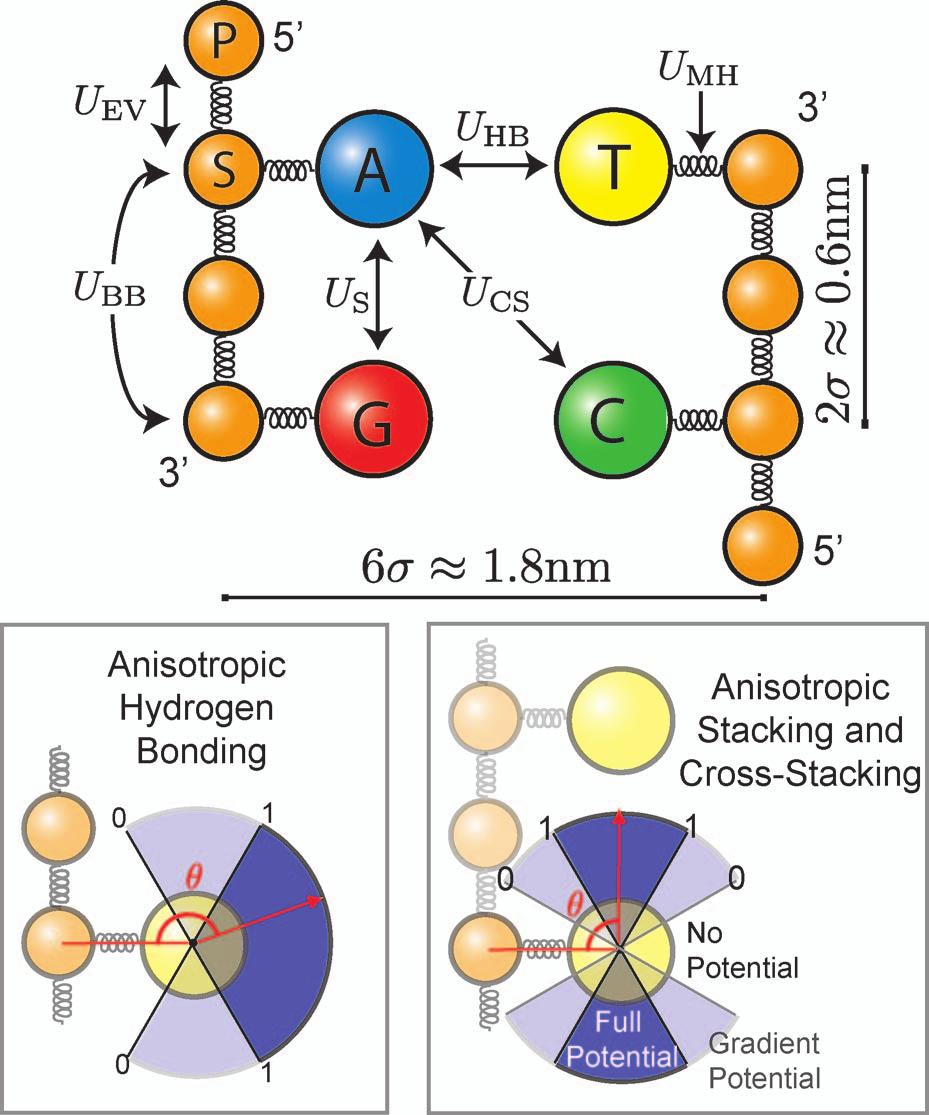
\includegraphics[width=0.6\textwidth]{moldyn.jpg}

\caption{Les différentes interactions modélisées}
\label{moldyn}
\end{center}
\end{figure}

Une fois ces potentiels calculés, ils sont sommés et dérivés afin d'être introduits dans l'équation de Langevin (7) qui est ensuite numériquement résolue.


\newpage 

\section{Expériences et utilisation du graphène}

Dans cette dernière partie, nous allons présenter le contexte expérimental dans lequel notre étude va se situer, les changements apportés par le graphène et la façon dont nous allons les modéliser.

\subsection{Courant de translocation et graphène}

La translocation d'ADN n'est pas un phénomène nouveau, et l'idée même de pouvoir s'en servir à des fins de séquençage a plus d'une quinzaine d'années \cite{holesedge}. L'idée est de mesurer le courant ionique à travers le pore lors de la translocation. Ce courant dépend de l'occupation ou non et de la nature de l'occupant du pore.\\

Dans les travaux précédents utilisant des bio-pores \cite{graph}, la taille du pore était un obstacle majeur. En effet, l'épaisseur du pore ayant la taille d'une centaine de paire de bases (environ $30$ $ nm$), le courant mesuré ne permettait pas de distinguer les séquences les unes des autres. Néanmoins la nature et la conformation de l'objet en translocation pouvaient être déterminées (protéine, ADN, ARN ...).\\

La récente utilisation du graphène permet de surmonter ce problème d'épaisseur puisqu'une mono-couche de graphène ne mesure que $0,3$ $ nm$.\\

La Figure \ref{courant} représente une vue d'artiste d'un système de séquençage utilisant le graphène:

\begin{figure}[H]
\begin{center}
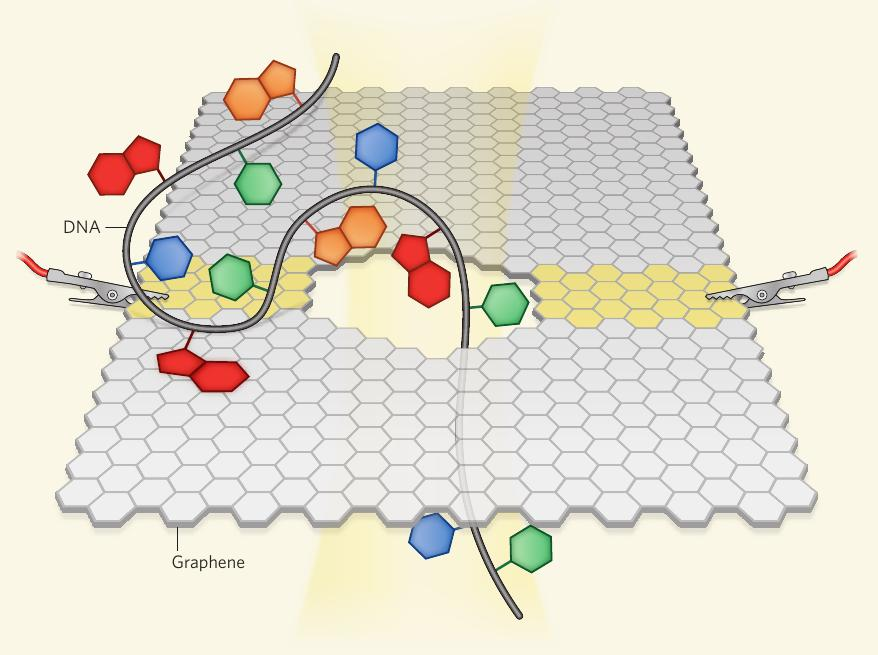
\includegraphics[width=0.5\textwidth]{courant.jpg}

\caption{Vers l'utilisation du graphène pour séquencer l'ADN en mesurant le courant de translocation.}
\label{courant}
\end{center}
\end{figure}


\subsection{Vers la modélisation du graphène}

Nous venons de voir que le graphène présente un potentiel intéressant afin de séquencer l'ADN, il faut maintenant s'interroger sur la façon dont nous allons le modéliser.\\

La première partie consiste à modéliser le graphène en lui même, faudra-t-il modéliser chaque atome, chaque cycle de six atomes, ou des ensembles de cycles ? Puisque la flexibilité du plan de graphène sera un élément clé, cette étape ne doit pas être survolée.\\

La seconde partie de la modélisation va consister en la description des interactions, au sein du graphène et avec les différents éléments du polymère. Il faudra notamment prendre en compte les interactions hydrophobe, d'éventuelles interactions électrostatiques, voir même des interactions hydrodynamiques. Toutes ces interactions vont demander beaucoup de ressources informatiques et il faudra donc étudier leurs importances relatives afin de ne pas surcharger le modèle (une réflexion aura lieu sur la nécessité de prendre en compte les liaisons hydrogènes par exemple). On pourra également s'inspirer de travaux récents \cite{doublebrin}.

\section{Conclusion}

Nous avons vu, dans la première partie, le comportement théorique d'un polymère et ce notamment lors de la translocation à travers un pore. Les outils analytiques développés vont permettre d'aider au développement et d'avoir un point de vue critique sur les résultats que nous obtiendrons avec une modélisation de type dynamique moléculaire introduite en seconde partie. Nous espérons que nos résultats permettront de relever les défis envisageables grâce aux récentes avancées expérimentales présentées en dernière section.\\

Nous nous attacherons particulièrement à déterminer les paramètres influant sur le temps de translocation, à étudier l'influence du graphène, notamment la flexibilité du plan et à discuter d'une éventuelle possibilité de séquencer l'ADN.

\bibliography{biblio}

\bibliographystyle{ieeetr}






\end{document}

